\documentclass{standalone}
\usepackage{tikz}
\begin{document}
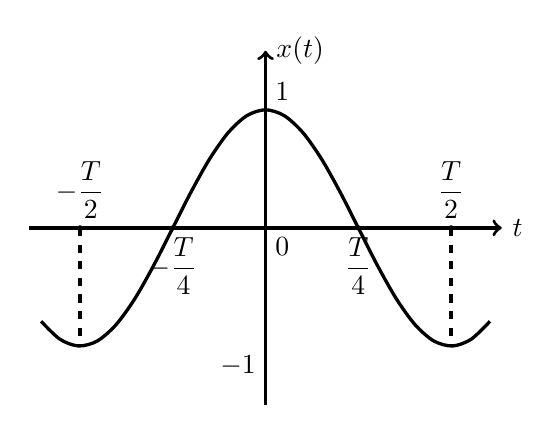
\begin{tikzpicture}[scale=1.5]
    \draw[->,very thick](0,-1.5)--(0,1.5)node[right]{$x(t)$};
    \draw[->,very thick](-2,0)--(2,0)node[right]{$t$};   
    \draw[-,very thick]plot[smooth, domain=-1.9:1.9](\x,{cos(2*\x r)});
    
    \node[below]at(0.785,0){$\displaystyle\frac{T}{4}$};
    \node[below]at(-0.785,0){$\displaystyle-\frac{T}{4}$};
    \node[above]at(1.5707,0){$\displaystyle\frac{T}{2}$};
    \node[above]at(-1.5707,0){$\displaystyle-\frac{T}{2}$};
    \draw[dashed,very thick](1.5707,0)--(1.5707,-1);
    \draw[dashed,very thick](-1.5707,0)--(-1.5707,-1);
    \node[above right]at(0,1){$1$};
    \node[below left]at(0,-1){$-1$};
    \node[below right]at(0,0){$0$};
    \filldraw[black](0.785,0)circle(0.5pt);
    \filldraw[black](-0.785,0)circle(0.5pt);
    \filldraw[black](1.5707,0)circle(0.5pt);
    \filldraw[black](-1.5707,0)circle(0.5pt);
\end{tikzpicture}
\end{document}